\begin{figure}[H]
\centering
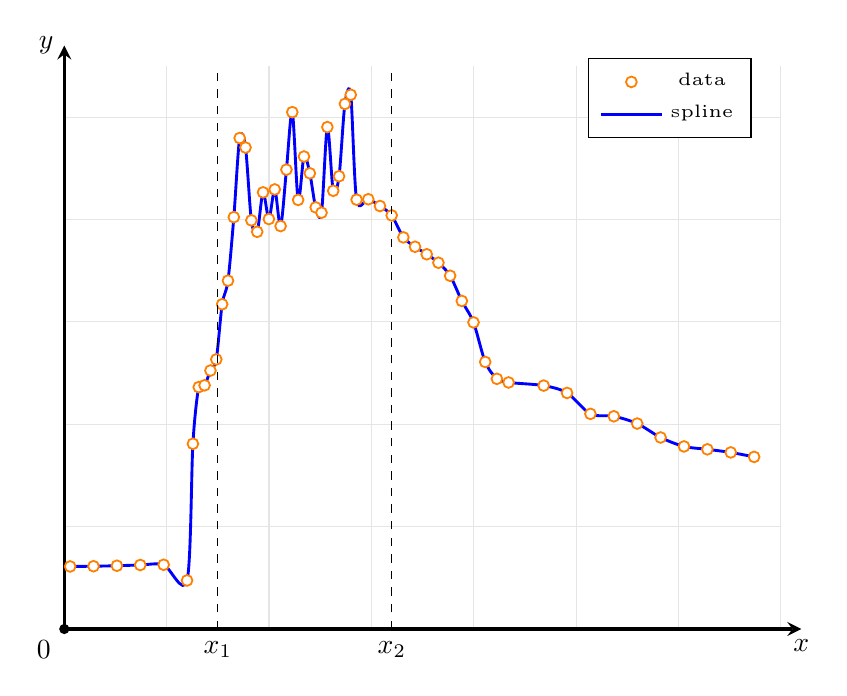
\begin{tikzpicture}[
	scale=1.3,
	axis/.style={
		-stealth,
		very thick
	}
]
% Gitter
\draw[gray!20] (0,0) grid (7,5.5);

% Achsen
\draw[axis] (0,0) -- (0,5.7) node[left]{$\boldsymbol{y}$};
\draw[axis] (0,0) -- (7.2,0) node[below]{$\boldsymbol{x}$};
\fill[black] (0,0) circle[radius=0.05];
\node at(-0.2,-0.2){$\boldsymbol{0}$};
	\begin{axis}[axis lines=none, xmin=40, xmax=160, mark size=1.5pt, legend style={font=\tiny}]
	%\pgfplotstableread{data/data.txt}
	%\datatable
	\addplot [mark=*,
			  only marks,
			  mark options={line width=0.5pt, color=orange,fill=white}]
                coordinates{
                (41,0.06030273)(45,0.10046387)(49,0.18066406)(53,0.30114746)(57,0.34130859)(61,-2.25805664)(62,20.40356445)(63,29.79736328)(64,30.09851074)(65,32.54736328)(66,34.39404297)(67,43.53698730)(68,47.45104980)(69,57.97900391)(70,71.09619141)(71,69.52062988)(72,57.44702148)(73,55.55017090)(74,62.09375000)(75,57.66784668)(76,62.57556152)(77,56.50366211)(78,65.85742188)(79,75.39172363)(80,60.83923340)(81,68.03527832)(82,65.25524902)(83,59.60485840)(84,58.72167969)(85,72.91284180)(86,62.35473633)(87,64.76342773)(88,76.75659180)(89,78.27209473)(90,60.87939453)(92,60.94970703)(94,59.82568359)(96,58.27001953)(98,54.62695312)(100,53.07128906)(102,51.82678223)(104,50.42175293)(106,48.26391602)(108,44.08886719)(110,40.52612305)(112,33.97241211)(114,31.17236328)(116,30.57019043)(122,30.04833984)(126,28.83398438)(130,25.36145020)(134,24.95996094)(138,23.75561523)(142,21.44738770)(146,19.96203613)(150,19.48022461)(154,18.96838379)(158,18.22570801)
                };
                \addlegendentry{data}
    
    \addplot [smooth,
			  color=blue,
			  thick]
                coordinates{
                (41,0.06030273)(45,0.10046387)(49,0.18066406)(53,0.30114746)(57,0.34130859)(61,-2.25805664)(62,20.40356445)(63,29.79736328)(64,30.09851074)(65,32.54736328)(66,34.39404297)(67,43.53698730)(68,47.45104980)(69,57.97900391)(70,71.09619141)(71,69.52062988)(72,57.44702148)(73,55.55017090)(74,62.09375000)(75,57.66784668)(76,62.57556152)(77,56.50366211)(78,65.85742188)(79,75.39172363)(80,60.83923340)(81,68.03527832)(82,65.25524902)(83,59.60485840)(84,58.72167969)(85,72.91284180)(86,62.35473633)(87,64.76342773)(88,76.75659180)(89,78.27209473)(90,60.87939453)(92,60.94970703)(94,59.82568359)(96,58.27001953)(98,54.62695312)(100,53.07128906)(102,51.82678223)(104,50.42175293)(106,48.26391602)(108,44.08886719)(110,40.52612305)(112,33.97241211)(114,31.17236328)(116,30.57019043)(122,30.04833984)(126,28.83398438)(130,25.36145020)(134,24.95996094)(138,23.75561523)(142,21.44738770)(146,19.96203613)(150,19.48022461)(154,18.96838379)(158,18.22570801)
                };
                \addlegendentry{spline}
	\end{axis}
	
	\node at(1.5,-0.2){$x_1$};
	\node at(3.2,-0.2){$x_2$};
	\draw[dashed] (1.5,0) -- (1.5,5.5);  
	\draw[dashed] (3.2,0) -- (3.2,5.5);  


\end{tikzpicture}
\caption[Graphische Darstellung der nichtparametrischen Regression]{Graphische Darstellung der nichtparametrischen Regression\protect\footnotemark}
\label{pr}
\end{figure}
\footnotetext{Abb. in Anlehnung an \textit{Günther}, Mathematische Modellbildung und Simulation, 2014, S. 92.}